
\documentclass[letterpaper,11pt]{article}

\usepackage{amsmath}
\usepackage{cite}
\usepackage[margin=1in]{geometry}
\usepackage{graphicx}
\usepackage{subfigure}
\usepackage{tikz}
\usepackage{url}
\usepackage{xspace}

\usetikzlibrary{fit}
\usetikzlibrary{positioning}
\usetikzlibrary{trees}

\tikzstyle{group}=[rectangle, rounded corners, thick, draw=green,
  minimum size=5ex, inner sep=1.5ex]
\tikzstyle{action}=[rectangle, rounded corners, thick, draw=blue,
  minimum size=5ex, inner sep=1.5ex]
\tikzstyle{object}=[rectangle, sharp corners, thick, draw=purple,
  minimum size=5ex, inner sep=1.5ex]
\tikzstyle{robject}=[object, anchor=east]


\tikzstyle{arrseq}=[->, >=stealth, thick, draw=blue]
\tikzstyle{arrdat}=[->, >=stealth, thick, dashed, draw=red]


\newcommand{\dealii}{\texttt{deal.II}\xspace}
\newcommand{\pforest}{\texttt{p4est}\xspace}

\newcommand{\figref}[1]{Figure~\ref{fig:#1}}

\author{Carsten Burstedde}
\title{Brief \pforest interface schematics}

\begin{document}

\maketitle

\begin{abstract}
We describe the general procedure of using \pforest from application codes.
\pforest is a software library that stores and modifies a forest-of-octrees
refinement structure using distributed (MPI) parallelism.  It expects the
description of the domain as a coarse mesh of conforming hexahedra.
Non-conforming adaptive mesh refinement (AMR), coarsening, and other operations
that modify the forest are implemented as \pforest API functions.  To inform
the application about the refinement structure, several methods are provided
that encode this information.
\end{abstract}

\section{Starting point}

We generally separate the adaptive mesh refinement (AMR) topology from any
numerical information.  The former is stored and modified internally by the
\pforest software library, while an application is free to define the way it
uses this information and arranges numerical and other data.  This document is
inteded to describe the interface by which \pforest relates mesh information
to the application.

The general, modular AMR pipeline is described in
\cite{BursteddeGhattasStadlerEtAl08}, which is not specific to \pforest but can
in principle be applied to any AMR provider.  The \pforest algorithms and main
interface routines are destribed in \cite{BursteddeWilcoxGhattas11}.
% \cite{IsaacBursteddeGhattas12}
An example usage of \pforest as scalable mesh backend for the general-purpose
finite element software \dealii is described in
\cite{BangerthBursteddeHeisterEtAl11}.  A reference implementation of \pforest
in \texttt{C} can be freely downloaded \cite{Burstedde10} and used and extended
under the GNU General Public License.  This code contains commented header
files and simple examples and use cases.  This software is best installed
standalone into a dedicated directory, where an application code can then find
the header and library files to compile and link against, respectively.

In this document, we document the three distinct tasks to
\begin{description}
\item[A] create a coarse mesh (\figref{partA}),
\item[B] modify the refinement and partition structure internal to \pforest
  (\figref{partB}),
\item[C] and to relate the mesh information to an application (\figref{partC}).
\end{description}
Unless indicated otherwise, all operations described below are understood as
MPI collectives, that is, they are called on all processors simultaneously.
Currently, part A needs to be performed redundantly on all processors, which is
acceptable for up to $10^5$--$10^6$ coarse cells (octree roots).  Parts B and C
strictly implement distributed parallelism, where runtime and per-processor
memory are roughly proportional to the number of local elements (octree leaves)
on a given processor, independent of the number of octrees, the total number of
elements, or the refinement depth.  Partitioning the forest into equal numbers
of elements per processor is a core \pforest operation and essentially free in
terms of execution time, so we suggest to call it whenever load balance is
desirable for subsequent operations.

\begin{figure}
\begin{center}
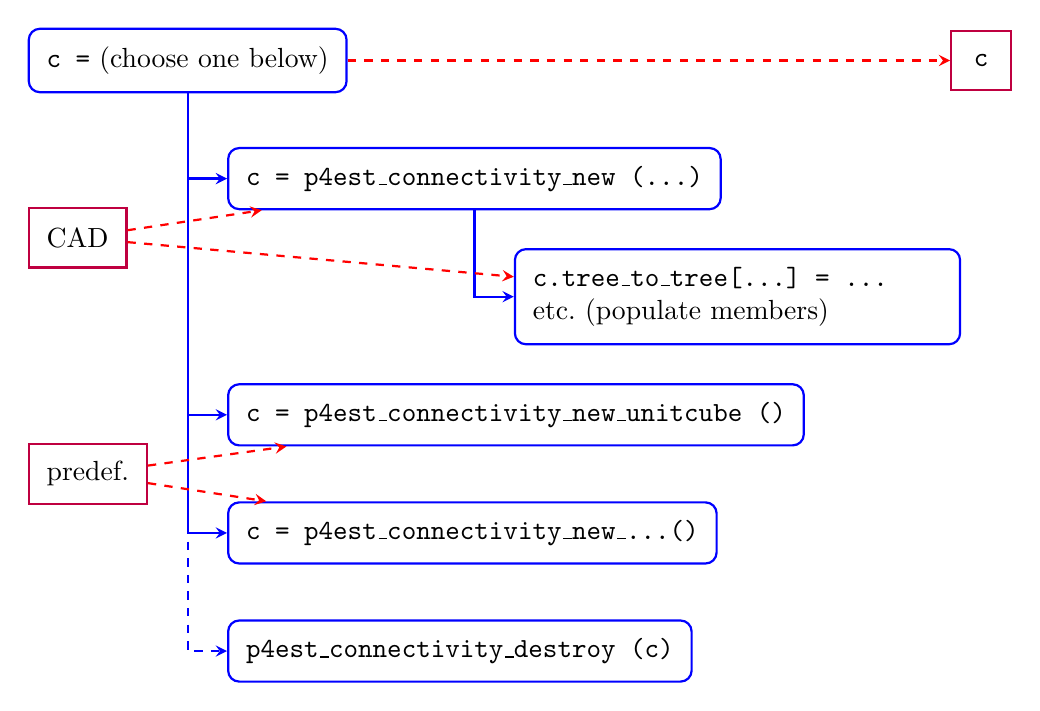
\begin{tikzpicture}[node distance=3ex,
  grow via three points = {one child at (0.5,-1.5) and
  two children at (0.5,-1.5) and (0.5,-3.0)},
  edge from parent path={(\tikzparentnode.south) |- (\tikzchildnode.west)}]

\tikzstyle{every node}=[action, anchor=west]
\tikzstyle{every child}=[arrseq]

\node (createconn) {\texttt{c =} (choose one below)}
child  {
%\node (CAD) {CAD / mesh generator / \ldots}
%  child {
  node (connnew) { \texttt{c = p4est\_connectivity\_new (\ldots)} }
  child {
    node (connfill) { \parbox{5.2cm}{\texttt{c.tree\_to\_tree[\ldots]~= \ldots}\\
                                   %\texttt{c\ldots}\\
                                   etc.\ (populate members)}}
  }
}
%\draw [arrseq] (CAD) -- (connnew);
%\draw [arrseq] (connnew) -- (connfill);
%\node[group, fit=(CAD) (connnew) (connfill)] (cadpipe) {};
child [missing] {}
child {
  node (newunit) { \texttt{c = p4est\_connectivity\_new\_unitcube ()} }
}
child {
  node (newstar) { \texttt{c = p4est\_connectivity\_new\_\ldots ()} }
}
child {
  node (conndestroy) { \texttt{p4est\_connectivity\_destroy (c)} }
  edge from parent[dashed]
};

\node[robject, xshift=12.5cm] (theconn) { \texttt{c} };
\draw[arrdat] (createconn) -- (theconn);
%\draw[arrdat] (newunit.east) -- (theconn);
%\draw[arrdat] (newstar.east) -- (theconn);

\node[object] at (0, -1.5-.75) (cadinput) {CAD};
\node[object] at (0, -4.5-.75) (predef) {predef.};

%\node[object, right=of theconn] (topartb) { Part B };
%\draw[arrdat, dashed] (theconn.east) -- (topartb.west);

%\draw[arrdat] (theconn) -- (conndestroy.east);
\draw[arrdat] (cadinput) -- (connnew);
\draw[arrdat] (cadinput) -- (connfill);
\draw[arrdat] (predef) -- (newunit);
\draw[arrdat] (predef) -- (newstar);

\end{tikzpicture}
\end{center}
\caption{Part A, creating the coarse mesh connectivity.  The \pforest connectivity
  \texttt{c} is a \texttt{C struct} that contains numbers and orientations of
  neighboring coarse cells.  It can be created by translating CAD or mesh data
  file formats or by using one of several predefined \pforest
  functions.  The data format is documented in the extensive comment blocks in
  \texttt{p4est\_connectivity.h} (2D) and \texttt{p8est\_connectivity.h} (3D);
  see also \cite{BursteddeWilcoxGhattas11}.
  In the following, \texttt{p4est} always refers to both 2D and 3D.
}%
\label{fig:partA}%
\end{figure}%

\begin{figure}
\begin{center}
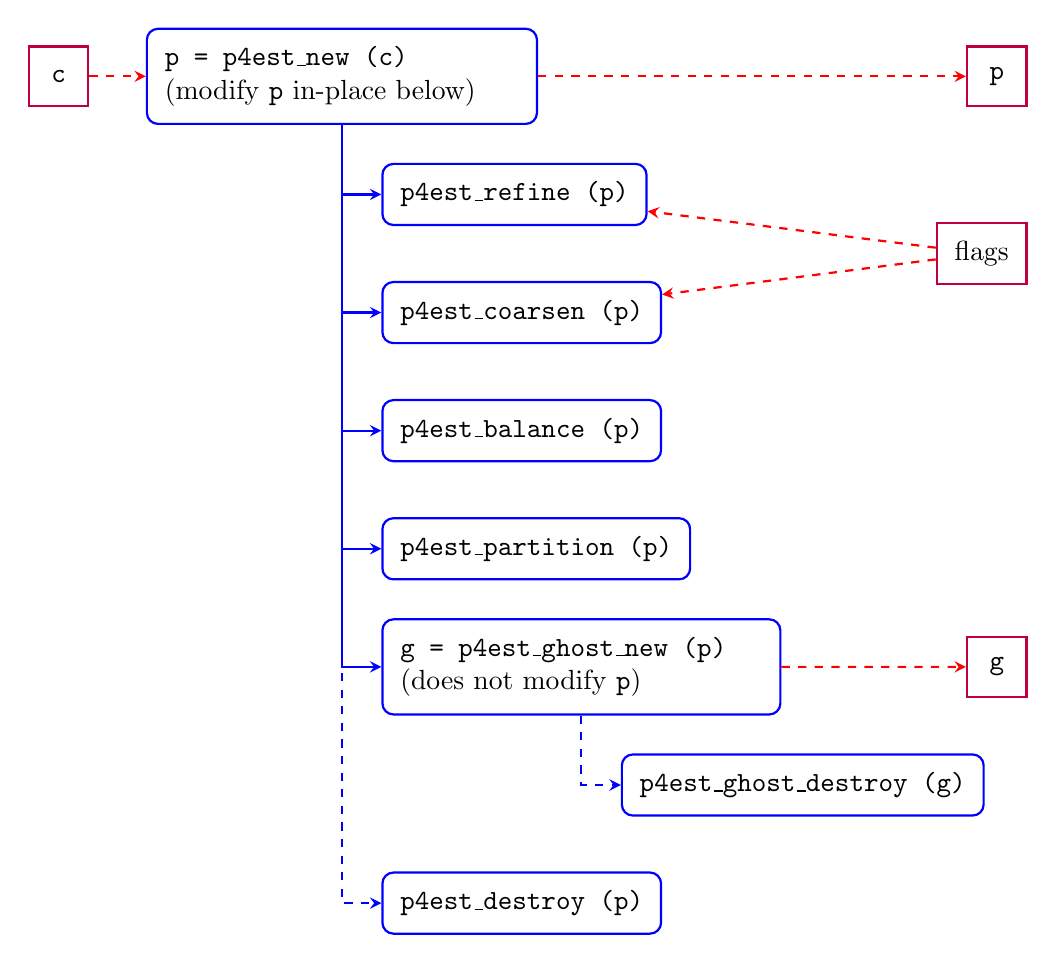
\begin{tikzpicture}[%node distance=3ex,
  grow via three points = {one child at (0.5,-1.5) and
  two children at (0.5,-1.5) and (0.5,-3.0)},
  edge from parent path={(\tikzparentnode.south) |- (\tikzchildnode.west)}]

\tikzstyle{every node}=[action, anchor=west]
\tikzstyle{every child}=[arrseq]

\node (p4estnew) {\parbox{4.5cm}{\texttt{p = p4est\_new (c)}\\
                                (modify \texttt{p} in-place below)}}
  child {
    node (p4estrefine) {\texttt{p4est\_refine (p)}}
  }
  child {
    node (p4estcoarsen) {\texttt{p4est\_coarsen (p)}}
  }
  child { 
    node (p4estbalance) {\texttt{p4est\_balance (p)}}
  }
  child {
    node (p4estpartition) {\texttt{p4est\_partition (p)}}
  }
  child {
    node (ghostnew) {\parbox{4.6cm}{\texttt{g = p4est\_ghost\_new (p)}\\
                                  (does not modify \texttt{p})}}
    child {
      node (ghostdestroy) {\texttt{p4est\_ghost\_destroy (g)}}
      edge from parent[dashed]
    }
  }
  child [missing] {}
  child {
    node (p4estdestroy) {\texttt{p4est\_destroy (p)}}
    edge from parent[dashed]
  };

\node[object, xshift=-1.5cm] (cinput) {\texttt{c}};
\draw[arrdat] (cinput) -- (p4estnew);

\node[robject, xshift=11.2cm] (poutput) {\texttt{p}};
\draw[arrdat] (p4estnew) -- (poutput);
\node[robject, xshift=11.2cm, yshift=-7.5cm] (goutput) {\texttt{g}};
\draw[arrdat] (ghostnew) -- (goutput);

\node[robject, xshift=11.2cm, yshift=-1.5cm-.75cm] (flags) {flags};
\draw[arrdat] (flags) -- (p4estrefine);
\draw[arrdat] (flags) -- (p4estcoarsen);

\end{tikzpicture}
\end{center}
\caption{Part B, changing the refinement structure and partition.  With the
  connectivity \texttt{c} created in part A, we can create the distributed
  \pforest structure.  Several functions for its modification exist.  For a
  given \pforest snapshot, we can create a ghost layer \texttt{g} of off-processor
  leaves, which will be outdated and should be destroyed once \texttt{p} is
  changed again.  Refinement and coarsening are controlled by callback functions
  that usually query flags
  determined by the application.  The \texttt{C struct}s \texttt{p} and \texttt{g}
  can be inspected directly by an application, for example to loop
  through data associated with local and ghost leaves.
}%
\label{fig:partB}%
\end{figure}%

\begin{figure}
\begin{center}
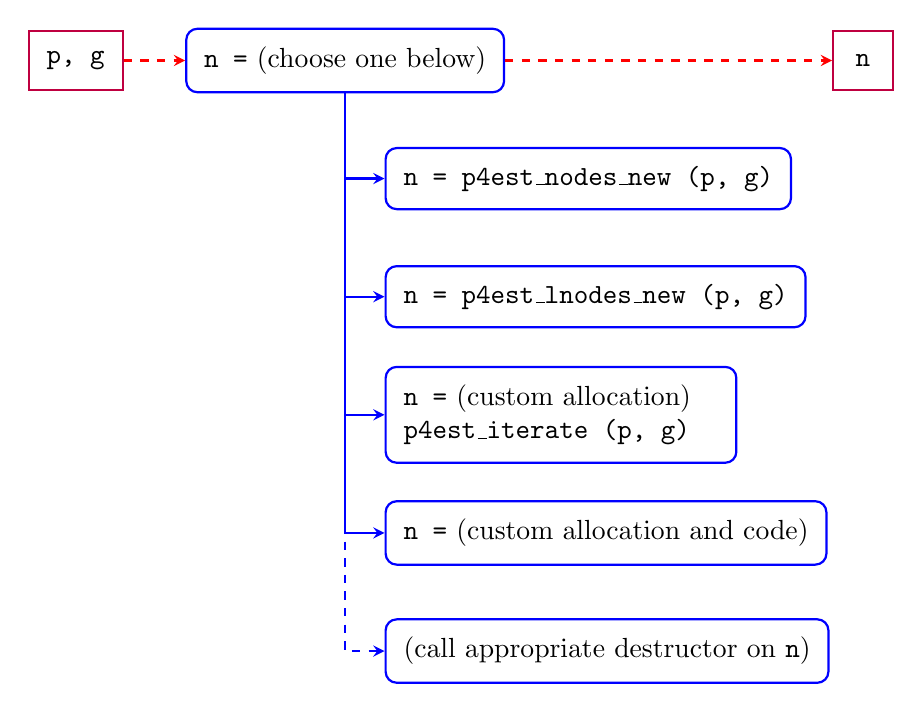
\begin{tikzpicture}[%node distance=3ex,
  grow via three points = {one child at (0.5,-1.5) and
  two children at (0.5,-1.5) and (0.5,-3.0)},
  edge from parent path={(\tikzparentnode.south) |- (\tikzchildnode.west)}]

\tikzstyle{every node}=[action, anchor=west]
\tikzstyle{every child}=[arrseq]

\node (createmesh) {%\parbox{8cm}{
\texttt{n =} %(numbering of degrees of freedom)\\
                                 (choose one below)}
  child {
    node (nodesnew) {\texttt{n = p4est\_nodes\_new (p, g)}}
  }
  child {
    node (lnodesnew) {\texttt{n = p4est\_lnodes\_new (p, g)}}
  }
  child {
    node (iterate) {\parbox{4cm}{\texttt{n =} (custom allocation)\\
      \texttt{p4est\_iterate (p, g)}}}
  }
  child {
    node (custom) {\texttt{n =} (custom allocation and code)}
  }
  child {
    node (ndestroy) {(call appropriate destructor on \texttt{n})}
    edge from parent[dashed]
  }
;

\node[object, xshift=-2.0cm] (pginput) {\texttt{p, g}};
\draw[arrdat] (pginput) -- (createmesh);

\node[robject, xshift=9.0cm] (themesh) {\texttt{n}};
\draw[arrdat] (createmesh) -- (themesh);

\end{tikzpicture}
\end{center}
\caption{Part C, creating an application-specific numbering of degrees of freedom.
  The \texttt{nodes} and \texttt{lnodes} constructors create a processor-local
  view of globally unique node numbers and the dependency lists for hanging
  nodes for continuous tensor-product piecewise linear and piecewise polynomial
  finite elements, respectively.  
  The iterator provides a generic way to traverse the refinement structure and to
  have callbacks executed for every face, edge, and corner neighborhood, which can
  then be used to identify node locations and their hanging status for any custom
  element type.  The \texttt{C}
  prototypes and documentation can be found in the respective \pforest
  \texttt{.h} files.%  Custom traversal and numbering can work as well.
}%
\label{fig:partC}%
\end{figure}%

\begin{figure}
\begin{center}
  \subfigure[Generating the initial refinement structure and mesh.]{%
  \includegraphics[width=.9\columnwidth]{plots/adaptivity/amr_octor1}%
  }
  \\
  \subfigure[A-posteriori change of refinement structure and mesh.]{%
  \includegraphics[width=.9\columnwidth]{plots/adaptivity/amr_octor2}%
  }
\end{center}
\caption{Separation between \pforest on one hand and application-specific mesh
  and numerical information on the other.
  The dark blue nodes in the picture correspond to in-place operations on the
  forest \texttt{p} that fall under part B (\figref{partB}).  The dark green node
  labeled
  ExtractMesh refers to creating a node numbering structure \texttt{n} (part C;
  see \figref{partC}) and the allocation of numerical space in application
  memory guided by \texttt{n}.  The bright green fields in the bottom-most row refer
  to moving the application-specific numerical information from the old mesh to
  the new one.  We suggest doing this in two steps: Interpolation works
  processor-local since the partition has not been changed at this point.
  Transfer moves data to the new owner processors of the respective degrees of
  freedom without changing the refinement pattern any further.  Both operations
  require the existence of both the old and
  new \texttt{n} structures, and allow for freeing the older one afterwards.
  (Plots originally published in \cite{BursteddeGhattasStadlerEtAl08}.)
}%
\label{fig:meshes}%
\end{figure}%

The definition and organisation of numerical data is entirely left up to the
application.  The application calls modification operations for the forest
(part B), guided by the numerical state related to the local leaves.  A
numerical application will require its own numbering scheme for degrees of
freedom, which is most of the time defined via node locations on a reference
element and dependencies between hanging nodes and the independent nodes they
are interpolated from.  \pforest provides several paths for aiding the
application in defining their data layout, henceforth called the mesh (part C),
and not to be confused with the coarse octree mesh (part A).  \figref{meshes}
contains illustrations on the sequence of operations that are required to
create a new refinement pattern from scratch or by modifying an existing one,
and to move the application-specific numerical data from an old to a new mesh.

\bibliographystyle{siam}
\bibliography{ccgo}

\end{document}
